\documentclass{standalone}

\usepackage{pgfgantt}

\def\pgfcalendarweekdayletter#1{%
  \ifcase#1M\or T\or W\or T\or F\or S\or S\fi%
}

\begin{document}
  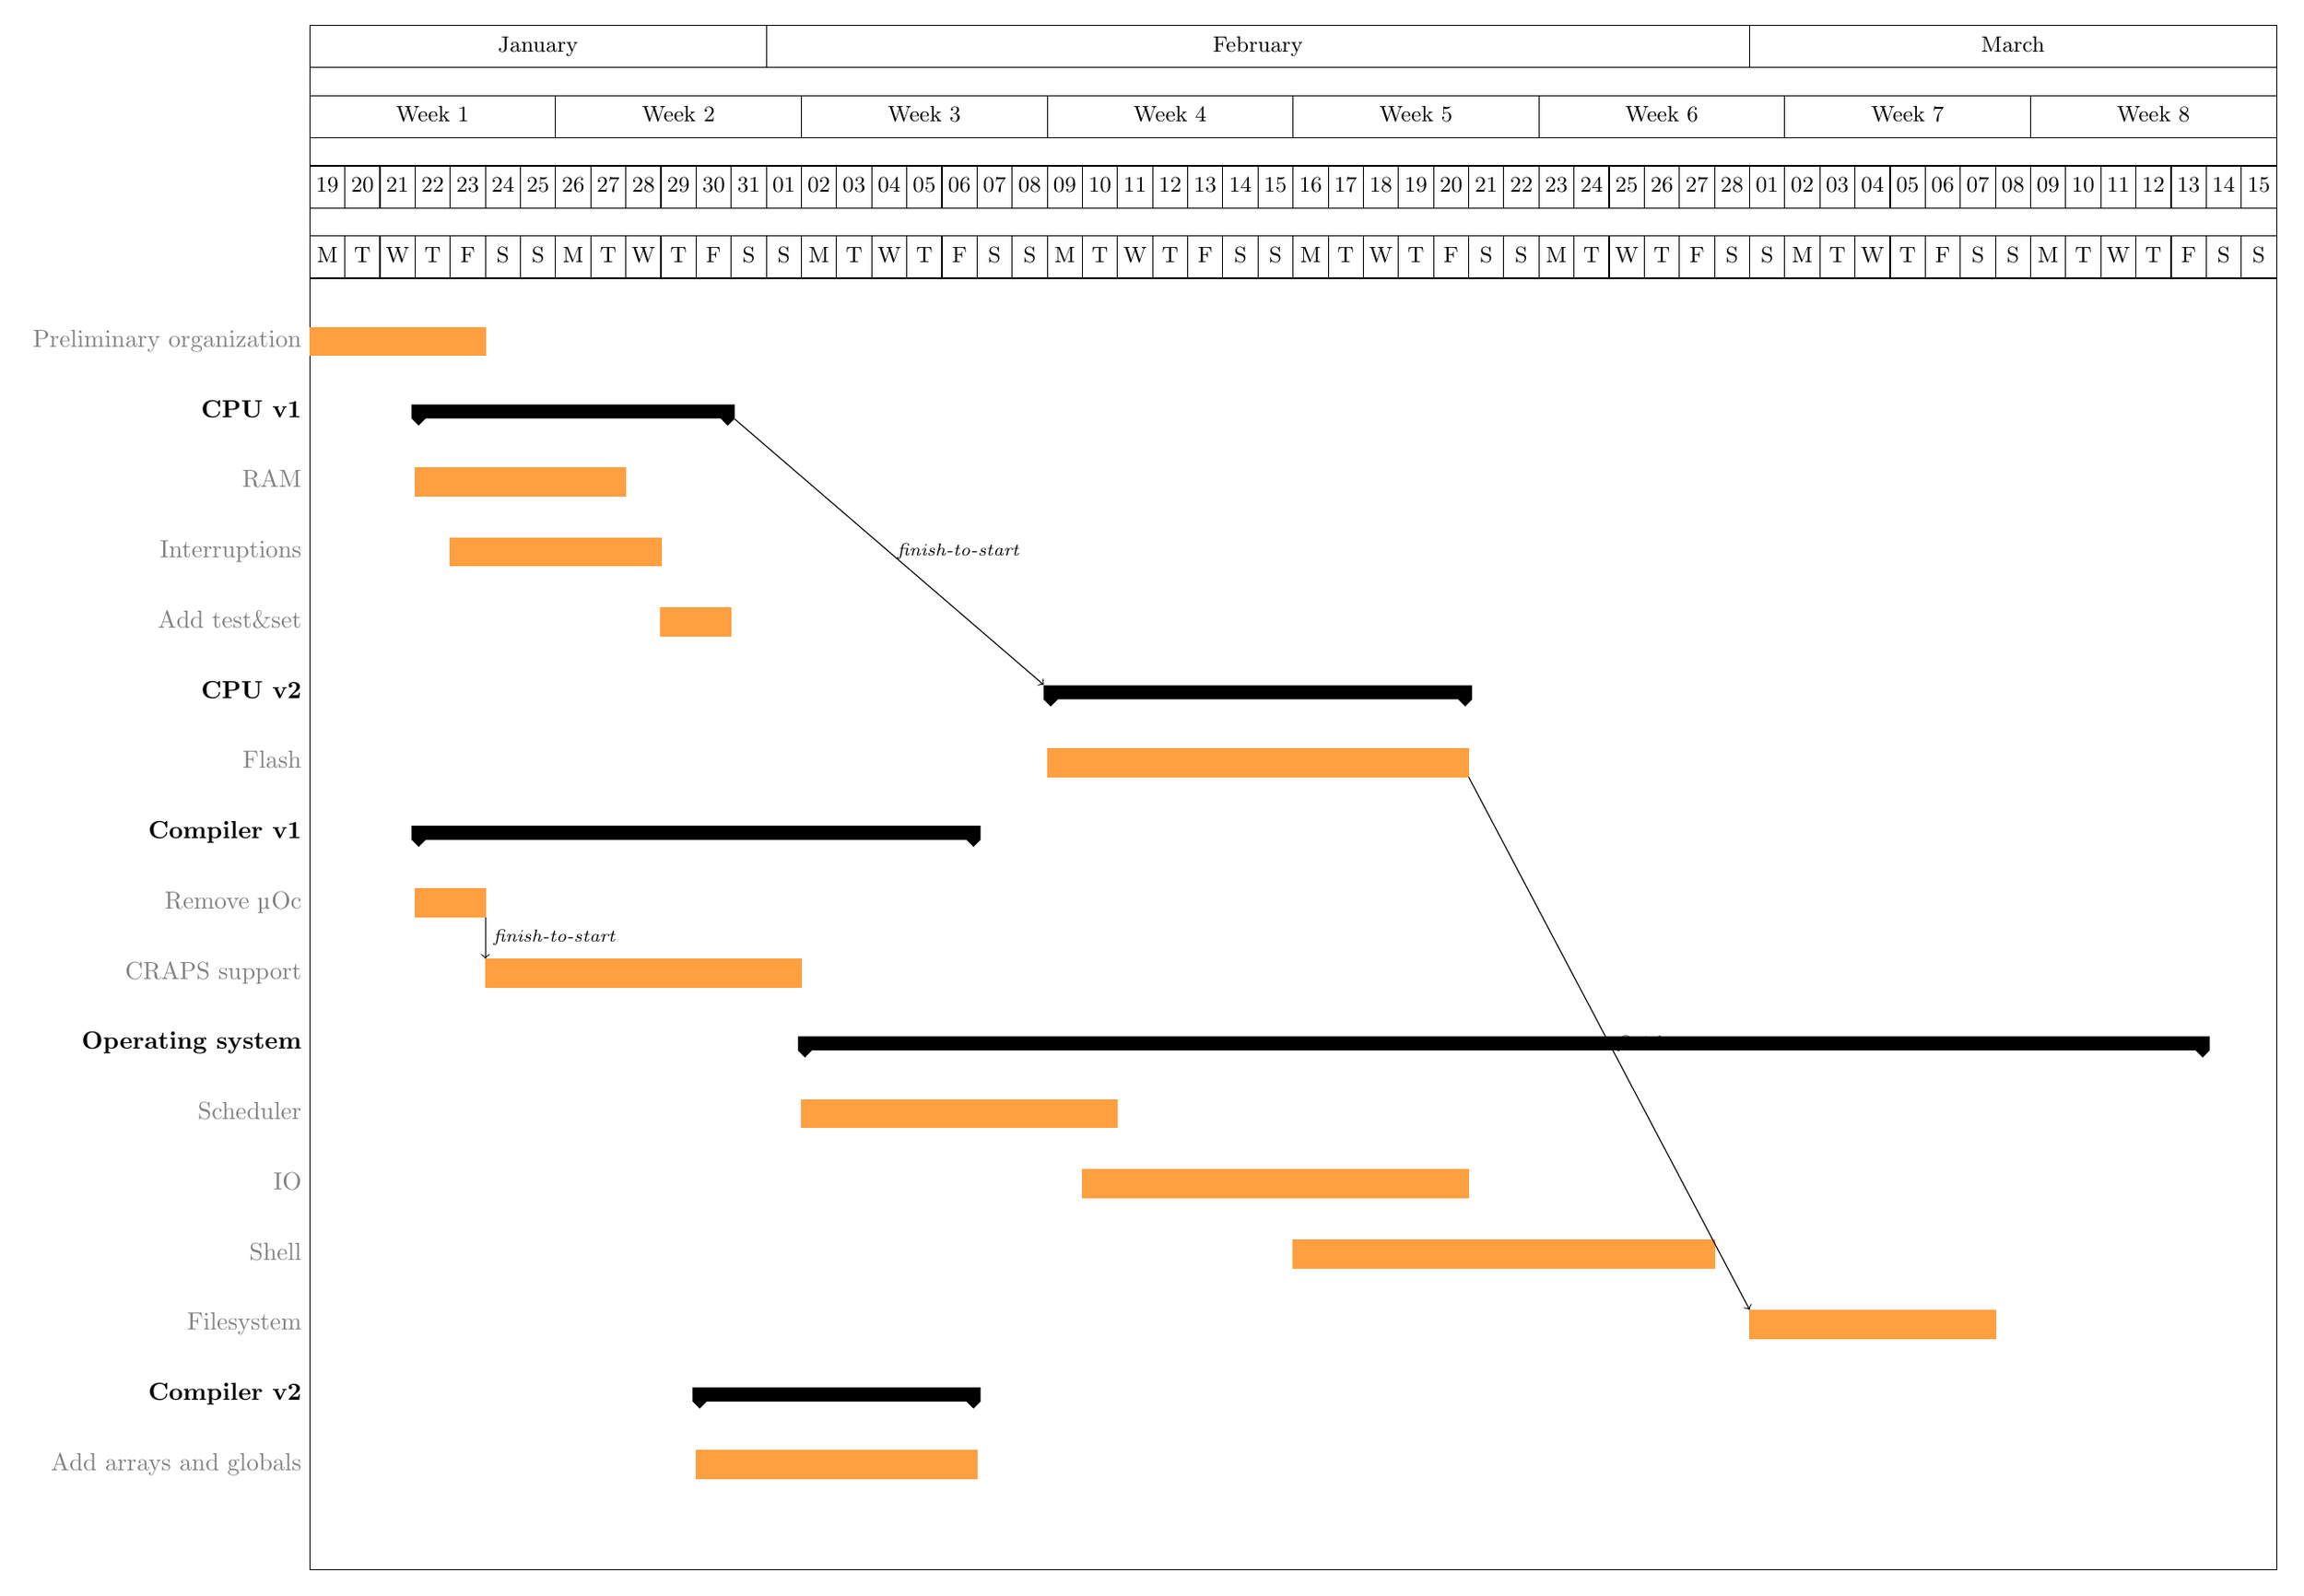
\begin{tikzpicture}
    \begin{ganttchart}[
        /pgf/outer xsep=+0pt,
        bar/.append style={orange!75},
        time slot format=isodate,
        link/.style={->},
        bar label font=\normalsize\color{black!50}
      ]{2015-01-19}{2015-03-15}
      \gantttitlecalendar{month=name, week, day, weekday=letter}            \\

      \ganttbar{Preliminary organization}{2015-01-19}{2015-01-23}           \\

      \ganttgroup[name=CPU1]{CPU v1}{2015-01-22}{2015-01-30}                \\
          \ganttbar[name=RAM]{RAM}{2015-01-22}{2015-01-27}                  \\
          \ganttbar[name=IT]{Interruptions}{2015-01-23}{2015-01-28}         \\
          \ganttbar{Add test\&set}{2015-01-29}{2015-01-30}                  \\

      \ganttgroup[name=CPU2]{CPU v2}{2015-02-09}{2015-02-20}                \\
          \ganttlink[link type=f-s]{CPU1}{CPU2}
          \ganttbar[name=flash]{Flash}{2015-02-09}{2015-02-20}              \\

      \ganttgroup[name=comp1]{Compiler v1}{2015-01-22}{2015-02-06}          \\
          \ganttbar[name=MOC]{Remove µOc}{2015-01-22}{2015-01-23}           \\
          \ganttbar[name=CRAPS]{CRAPS support}{2015-01-24}{2015-02-01}      \\

      \ganttgroup[name=os]{Operating system}{2015-02-02}{2015-03-13}        \\
          \ganttbar{Scheduler}{2015-02-02}{2015-02-10}                      \\
          \ganttbar{IO}{2015-02-10}{2015-02-20}                             \\
          \ganttbar{Shell}{2015-02-16}{2015-02-27}                          \\
          \ganttbar[name=FS]{Filesystem}{2015-02-29}{2015-03-07}            \\

          \ganttlink[link type=f-s]{flash}{FS}

      \ganttgroup[name=comp2]{Compiler v2}{2015-01-30}{2015-02-06}          \\
          \ganttbar{Add arrays and globals}{2015-01-30}{2015-02-06}         \\

          \ganttlink[link type=f-s]{MOC}{CRAPS}
    \end{ganttchart}
  \end{tikzpicture}
\end{document}
